% Template file for an a0 landscape poster.
% Written by Graeme, 2001-03 based on Norman's original microlensing
% poster.
%
% See discussion and documentation at
% <http://www.astro.gla.ac.uk/users/norman/docs/posters/> 
%
% $Id: poster-template-landscape.tex,v 1.2 2002/12/03 11:25:46 norman Exp $


% Default mode is landscape, which is what we want, however dvips and
% a0poster do not quite do the right thing, so we end up with text in
% landscape style (wide and short) down a portrait page (narrow and
% long). Printing this onto the a0 printer chops the right hand edge.
% However, 'psnup' can save the day, reorienting the text so that the
% poster prints lengthways down an a0 portrait bounding box.
%
% 'psnup -w85cm -h119cm -f poster_from_dvips.ps poster_in_landscape.ps'

\documentclass[a0]{a0poster}
% You might find the 'draft' option to a0 poster useful if you have
% lots of graphics, because they can take some time to process and
% display. (\documentclass[a0,draft]{a0poster})
\input defs
\pagestyle{empty}
\setcounter{secnumdepth}{0}
\renewcommand{\familydefault}{\sfdefault}
\newcommand{\QED}{~~\rule[-1pt]{8pt}{8pt}}\def\qed{\QED}

\renewcommand{\reals}{{\mbox{\bf R}}}

% The textpos package is necessary to position textblocks at arbitary 
% places on the page.
\usepackage[absolute]{textpos}

\usepackage{fleqn,psfrag,wrapfig,tikz}

\usepackage[papersize={38in,28in}]{geometry}

% Graphics to include graphics. Times is nice on posters, but you
% might want to switch it off and go for CMR fonts.
\usepackage{graphics}



\usepackage{algorithm}
\usepackage{algorithmic}
\renewcommand{\algorithmicrequire}{\textbf{Input:}}
\renewcommand{\algorithmicensure}{\textbf{Output:}}

\usepackage{multirow}


% we are running pdflatex, so convert .eps files to .pdf
%\usepackage[pdftex]{graphicx}
%\usepackage{epstopdf}

% These colours are tried and tested for titles and headers. Don't
% over use color!
\usepackage{color}
\definecolor{Red}{rgb}{0.9,0.0,0.1}

\definecolor{bluegray}{rgb}{0.15,0.20,0.40}
\definecolor{bluegraylight}{rgb}{0.35,0.40,0.60}
\definecolor{gray}{rgb}{0.3,0.3,0.3}
\definecolor{lightgray}{rgb}{0.7,0.7,0.7}
\definecolor{darkblue}{rgb}{0.2,0.2,1.0}
\definecolor{darkgreen}{rgb}{0.0,0.5,0.3}

\renewcommand{\labelitemi}{\textcolor{bluegray}\textbullet}
\renewcommand{\labelitemii}{\textcolor{bluegray}{--}}

\setlength{\labelsep}{0.5em}


% see documentation for a0poster class for the size options here
\let\Textsize\normalsize
%\def\Head#1{\noindent\hbox to \hsize{\hfil{\LARGE\color{bluegray} #1}}\bigskip}
\def\Head#1{\noindent{\LARGE\color{bluegray} #1}\bigskip}
\def\LHead#1{\noindent{\LARGE\color{bluegray} #1}\bigskip}
\def\Subhead#1{\noindent{\large\color{bluegray} #1}\bigskip}
\def\Title#1{\noindent{\VeryHuge\color{Red} #1}}


% Set up the grid
%
% Note that [40mm,40mm] is the margin round the edge of the page --
% it is _not_ the grid size. That is always defined as 
% PAGE_WIDTH/HGRID and PAGE_HEIGHT/VGRID. In this case we use
% 23 x 12. This gives us three columns of width 7 boxes, with a gap of
% width 1 in between them. 12 vertical boxes is a good number to work
% with.
%
% Note however that texblocks can be positioned fractionally as well,
% so really any convenient grid size can be used.
%
\TPGrid[40mm,40mm]{23}{12}      % 3 cols of width 7, plus 2 gaps width 1

\parindent=0pt
\parskip=0.2\baselineskip

\begin{document}

% Understanding textblocks is the key to being able to do a poster in
% LaTeX. In
%
%    \begin{textblock}{wid}(x,y)
%    ...
%    \end{textblock}
%
% the first argument gives the block width in units of the grid
% cells specified above in \TPGrid; the second gives the (x,y)
% position on the grid, with the y axis pointing down.

% You will have to do a lot of previewing to get everything in the 
% right place.

% This gives good title positioning for a portrait poster.
% Watch out for hyphenation in titles - LaTeX will do it
% but it looks awful.
\begin{textblock}{23}(0,0)
\Title{Stochastic Quasi Newton methods for Neural Networks}
\end{textblock}

\begin{textblock}{23}(0,0.6)
{
\LARGE
Konstantin Yakovlev
}

{
\Large
\color{bluegray}
\emph{Optimization Class Project. MIPT}
}
\end{textblock}


% Uni logo in the top right corner. A&A in the bottom left. Gives a
% good visual balance, but you may want to change this depending upon
% the graphics that are in your poster.
%\begin{textblock}{2}(0,10)
%Your logo here
%%\includegraphics{/usr/local/share/images/AandA.epsf}
%\end{textblock}

%\begin{textblock}{2}(21.2,0)
%Another logo here
%%\resizebox{2\TPHorizModule}{!}{\includegraphics{/usr/local/share/images/GUVIu/GUVIu.eps}}
%\end{textblock}


\begin{textblock}{7.0}(0,1.5)

\hrule\medskip
\Head{Introduction}\\
The project considers a stochastic quasi-Newtonian method. This project draws heavily on the work of \cite{journals/siamjo/ByrdHNS16}. The algorithm given here uses the classical BFGS update formula in its bounded form. It is also efficient, robust, scalable, and has promising prospects in machine learning. In this project, we propose to implement the above algorithm and compare it with the oBFGS \cite{journals/jmlr/SchraudolphYG07} algorithm on the example of logistic regression. In addition, we will compare two optimizers of a neural network -- SQGN \cite{journals/corr/abs-2004-03040} and SGD.

\medskip
\hrule\medskip
\Head{Problem statement}\\
%Problem statement from \cite{journals/siamjo/ByrdHNS16}. I'll try to compress it.
Let us give some function $f(w, \xi)$, where $w\in \reals^n, ~\xi$ is a random vector $(x, z)$. You can look at the pair $(x, z)$ as an object and an answer, respectively. Usually in machine learning, the function $f(w, \xi)$ has the form:
$$f(w, \xi) = \ell(h(w; x_i); z_i),$$
where $\ell$ is a non-negative loss function, $h$ is a model parameterized by the vector $w$, $\{x_i, z_i\}_{i=1}^N$ is a training sample. We define the empirical risk as:
$$F(w) = \frac{1}{N}\sum_{i=1}^Nf(w; x_i, z_i)$$

We formulate the optimization problem as follows:
$$\min_{w\in \reals^n}F(w)$$

One can give an estimate of the gradient and the hessian:
\begin{equation}
\label{risk_approx}
\widehat{\nabla}F(w) = \frac{1}{b}\sum_{i\in \mathcal{S}}\nabla f(w; x_i, z_i)
\end{equation}
\begin{equation}
\label{hess_risk_approx}
\widehat{\nabla}^2F(w) = \frac{1}{b_H}\sum_{i\in\mathcal{S}_H}\nabla^2f(w; x_i, z_i)
\end{equation}

%One approach is the \emph{group lasso}:
%\[
%\begin{array}{ll}
%\mbox{minimize} & f(x) + \lambda \sum_{i=1}^N \|x_i\|_2
%\end{array}
%\]
%\ie, like lasso, but require groups of variables to be zero or not
%\begin{itemize}\itemsep=12pt
%\item also called $\ell_{1,2}$ mixed norm regularization
%\end{itemize}

\medskip
\hrule\medskip
\Head{Stochastic quasi-Newton method}\\
%Description from \cite{journals/siamjo/ByrdHNS16}.
Let the optimization method have the following form:
\begin{equation}
\label{qn:iteration}
w^{k + 1} = w^k - \alpha^kH_k\widehat{\nabla}F(w^k)
\end{equation}
We introduce the following notation:

$$s_t = \overline{w} _t- \overline{w}_{t-1}, \quad \overline{w}_t = \sum_{i = k-L}^kw^i, \quad y_t = \widehat{\nabla}^2F(\overline{w}_t)s_t$$

Let us define the $H_k$ update:

$$H_{k+1} = (I -\rho_ks_ky_k^\top)H_k(I - \rho_ky_ks_k^\top) + \rho_ks_ks_k^\top, \quad \rho_k = \frac{1}{y_k^\top s_k}$$

%Another approach is the \emph{structured group lasso}:
%\[
%\begin{array}{ll}
%\mbox{minimize} & f(x) + \sum_{i=1}^N \lambda_i \|x_{g_i}\|_2
%\end{array}
%\]
%where $g_i \subseteq [n]$ and $\mathcal G = \{g_1, \dots, g_N\}$
%\begin{itemize}\itemsep=12pt
%\item like group lasso, but the groups can overlap arbitrarily
%\item particular choices of groups can impose `structured' sparsity
%\item \eg, topic models, selecting interaction terms for (graphical) models,
%    tree structure of gene networks, fMRI data
%\item generalizes to the \textbf{composite absolute penalties family}:
%\[
%r(x) = \|(\|x_{g_1}\|_{p_1}, \dots, \|x_{g_N}\|_{p_N})\|_{p_0}
%\]
%\end{itemize}
\end{textblock}

\begin{textblock}{7.0}(8,1.5)

Vectors $s_t$ and $y_t$ are calculated every $L$ iterations, where $L$ is a positive integer.

In addition, updating the weights on the iteration number $k \leq 2L$ has the following form:

$$w^{k+1} = w^k - \alpha_k\widehat{\nabla}F(w^k)$$
%\hrule\medskip
%\Head{Algorithm}\\
%The algorithms is described in the project proposal.
%\begin{algorithm}[!h]
%		\caption{Stochastic Quasi-Newton Method (SQN)}	
%SQN
%	\begin{algorithmic}[1]
%	\label{SQN}
%		\REQUIRE initial parameters $w^1$; positive integers $M, L$; step-length sequence $\{\alpha_k\}$
%		\STATE Set $t = -1$
%		\STATE Set $\overline{w}_t = 0$		
%		\FOR {$k=1,2,...,$}
%		\STATE Choose a sample $\mathcal S \subset\{1, \ldots, N\}$
%		\STATE Calculate $\widehat{\nabla}F(w^k)$ as defined in \ref{risk_approx}
%		\STATE $\overline{w}_t = \overline{w}_t + w^k$
%		\IF {$k\leq 2L$}
%			\STATE $w^{k+1} = w^k - \alpha_k \widehat{\nabla}F(w^k)$
%		\ELSE 
%			\STATE $w^{k+1} = w^k - \alpha_kH_t\widehat{\nabla}F(w^k)$, $H_t$ is defined by \ref{hess_updating}
%		\ENDIF
%		
%		\IF {$k ~\%~ L = 0$}
%			\STATE $t = t+1$
%			\STATE $\overline{w}_t = \overline{w}_t / L$
%			\IF {$t > 0$}
%				\STATE Choose a sample $\mathcal{S}_H \subset \{1,\ldots,N\}$, to define $\widehat{\nabla}^2F(\overline{w}_t)$ by \ref{hess_risk_approx}
%				 \STATE Compute $s_t = \overline{w}_t - \overline{w}_{t-1}, ~y_t = \widehat{\nabla}^2F(\overline{w}_t)(\overline{w}_t - \overline{w}_{t-1})$ \label{st_yt}
%			\ENDIF
%			\STATE $\overline{w}_t = 0$
%		\ENDIF
%		\ENDFOR
%	\end{algorithmic}
%%\end{algorithm}
%
%%\begin{algorithm}[H]
%%	\caption{Обновление Гессиана}
%Hessian updating
%	\begin{algorithmic}[1]
%		\label{hess_updating}
%	\REQUIRE Updating counter $t$, memory parameter $M$ , and correction pairs $(s_j, y_j)$,\\$j = t - \min(t, M) + 1, \ldots, t$
%	\ENSURE $H_t$
%	\STATE Initialize $H = (s_t^\top y_t)/(y_t^\top y_t)I$, where $s_t, y_t$ are computed in Step \ref{st_yt} of \ref{SQN}
%	\FOR {$j = t - \min(t, M) + 1, \ldots, t$}
%		\STATE $\rho_j = 1/y_j^\top s_j$
%		\STATE Apply BFGS formula: $H_t = (I - \rho_js_jy_j^\top)H(I - \rho_jy_js_j^\top) + \rho_js_js_j^\top$
%	\ENDFOR
%	\RETURN $H_t$
%	\end{algorithmic}
%%\end{algorithm}


%\begin{center}
%\begin{tikzpicture}
%[dot/.style={rectangle,draw=black,fill=white,inner sep=5pt,minimum size=5pt}]
%\node[dot,draw=orange,thick] at (0,10) (n1) {1};
%\node[dot] at (-3,8) (n2) {2};
%\node[dot,draw=orange,thick] at (3,8) (n3) {3};
%\node[dot] at (-3,6) (n4) {4};
%\node[dot,draw=orange,thick] at (1.5,6) (n5) {5};
%\node[dot] at (4.5,6) (n6) {6};
%\draw[->] (n1) -- (n2);
%\draw[->] (n1) -- (n3);
%\draw[->] (n2) -- (n4);
%\draw[->] (n3) -- (n5);
%\draw[->] (n3) -- (n6);
%\end{tikzpicture}
%\end{center}
%
%\begin{itemize}\itemsep=8pt
%    \item $\mathcal G = \{ \{4\}, \textcolor{orange}{\{5\}}, \{6\}, \{2,4\}, 
%        \textcolor{orange}{\{3,5,6\}}, \textcolor{orange}{\{1,2,3,4,5,6\} \}}$
%\item nonzero variables form a rooted and connected subtree
%    \begin{itemize}
%        \item if node is selected, so are its ancestors
%        \item if node is not selected, neither are its descendants
%    \end{itemize}
%\end{itemize}


\hrule\medskip
\Head{Convergence}\\
%Theorem from \cite{journals/siamjo/ByrdHNS16}
Suppose that $F(w)$ is twice continuously differentiable. There exist positive constants $\lambda$ and $\Lambda$ such that, for all $w\in \reals^n \hookrightarrow \lambda I \prec \nabla^2F(w)\prec \Lambda$. There is a constant $\gamma$ such that, for all $w\in \reals^n \hookrightarrow E_\xi[\|\nabla f(w^k, \xi)\|_2]^2 \leq \gamma^2$. For convenience, we define $\alpha^k = \frac{\beta}{k}$. Let $w^k$ be the iterates generated by the Newton-like method \ref{qn:iteration}. Where for all $k$ made:
$$\mu_1I\prec H_k \prec \mu_2I, ~0 < \mu_1 \leq \mu_2, ~\beta > (2\mu_1\lambda)^{-1}$$
Then, for all $k\geq 1$
$$E[F(w^k) - F(w_*)] \leq \frac{Q(\beta)}{k}, ~ Q(\beta) = \max\left(\frac{\Lambda\mu_2^2\beta^2\gamma^2}{2(2\mu_1\lambda\beta - 1)}, F(w^1) - F(w_*)\right)$$

%We solve this problem using an ADMM lasso implementation:
%\begin{verbatim}
%prox_f = @(v,rho) (rho/(1 + rho))*(v - b) + b;
%prox_g = @(v,rho) (max(0, v - 1/rho) - max(0, -v - 1/rho));
%
%AA = A*A';
%L  = chol(eye(m) + AA);
%
%for iter = 1:MAX_ITER
%    xx = prox_g(xz - xt, rho);
%    yx = prox_f(yz - yt, rho);
%
%    yz = L \ (L' \ (A*(xx + xt) + AA*(yx + yt)));
%    xz = xx + xt + A'*(yx + yt - yz);
%  
%    xt = xt + xx - xz;
%    yt = yt + yx - yz;
%end
%\end{verbatim}

\hrule\medskip
\Head{Basic experiment}\\
Here we considered the classification problem, but also the logistic regression. Two optimizers were compared: oLBFGS \cite{journals/jmlr/SchraudolphYG07} and SQN \cite{journals/siamjo/ByrdHNS16} on a digits dataset from sklearn library.

\begin{center}
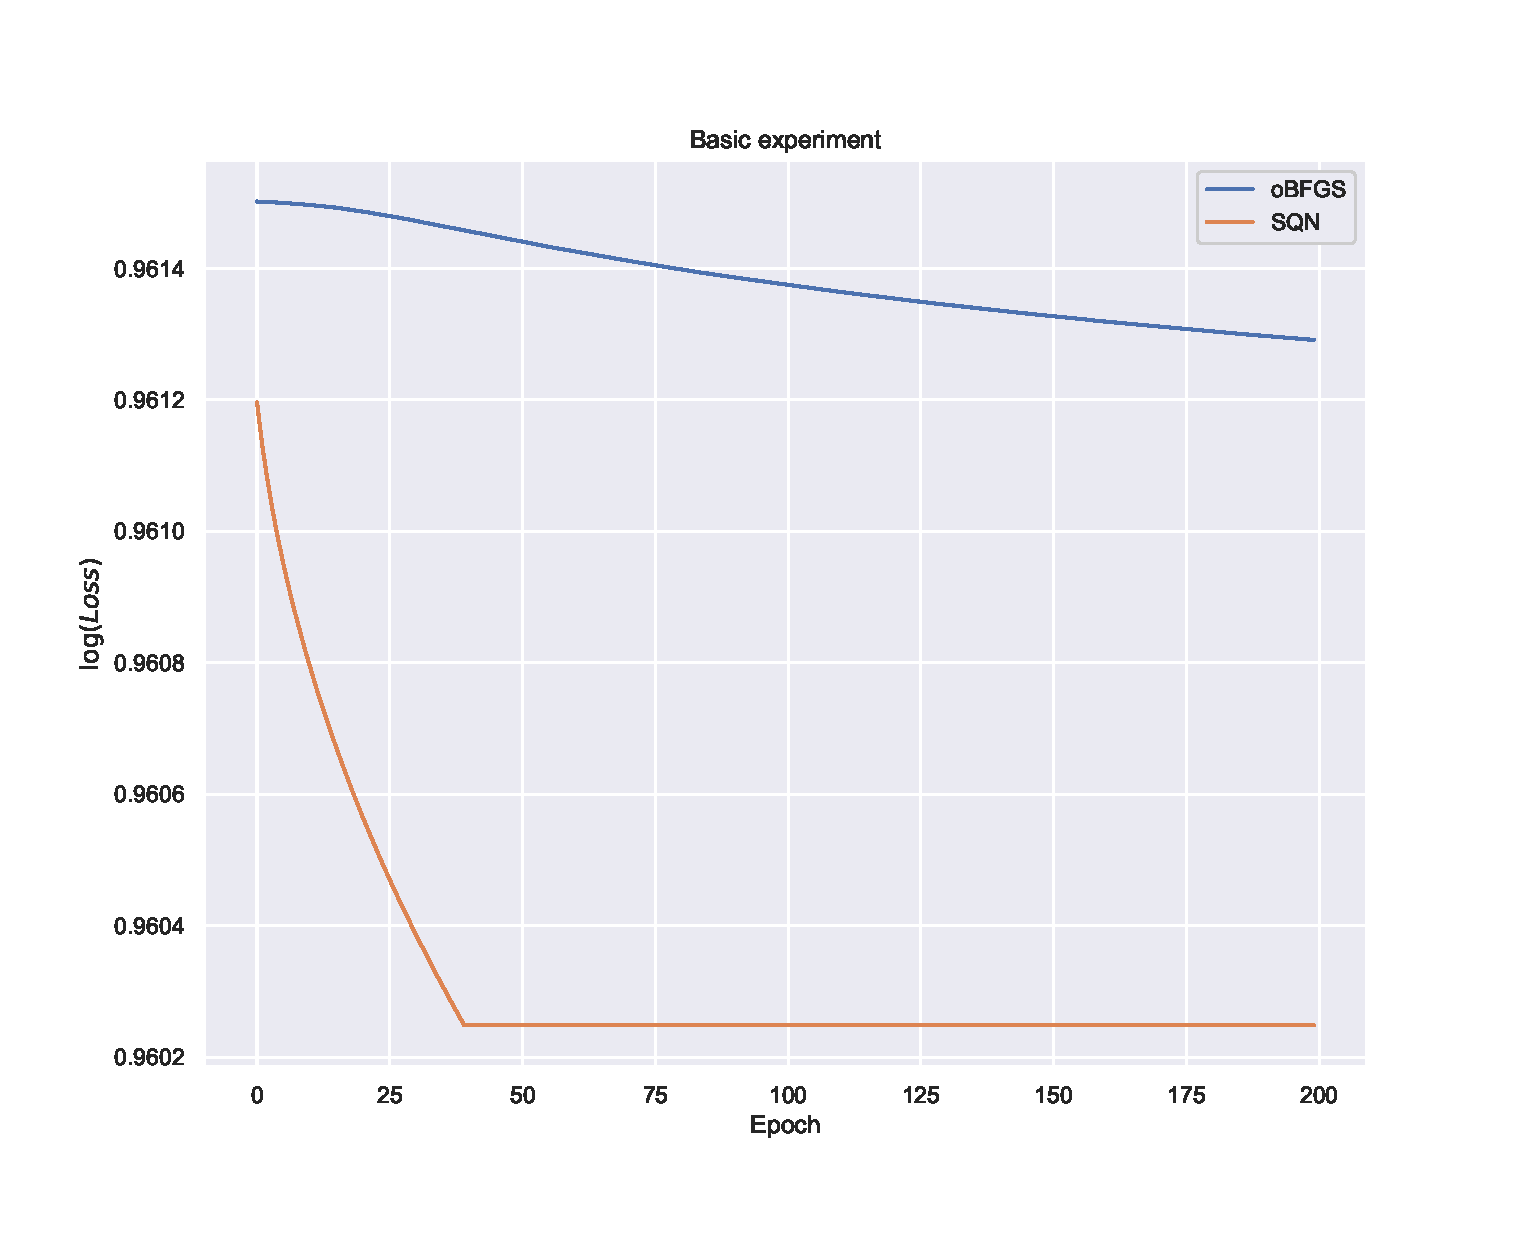
\includegraphics[width=0.9\textwidth]{basic_exp.eps}
\end{center}
%If $L$ is not known (usually the case), can use the following line search:
%
%\noindent\rule[-5pt]{.8\textwidth}{0.4pt}
%{\footnotesize
%\begin{tabbing}
%    {\bf given} $x^k$, $\lambda^{k-1}$, and parameter $\beta \in (0,1)$. \\*[\smallskipamount]
%    Let $\lambda := \lambda^{k-1}$. \\*[\smallskipamount]
%    {\bf repeat} \\
%    \qquad \= 1.\ Let $z := \prox_{\lambda g}(x^{k} - \lambda \nabla f(x^{k}))$. \\
%    \> 2.\ {\bf break if} $f(z) \leq \hat{f}_{\lambda}(z, x^{k})$. \\
%    \> 3.\ Update $\lambda := \beta \lambda$. \\*[\smallskipamount]
%    {\bf return} $\lambda^{k} := \lambda$, $x^{k+1}:=z$.
%\end{tabbing}}
%\noindent\rule[10pt]{.8\textwidth}{0.4pt}
%
%typical value of $\beta$ is $1/2$, and 
%\[
%\hat{f}_\lambda(x,y) = f(y) + \nabla f(y)^T (x - y) + 
%(1/2\lambda)\|x - y\|_2^2
%\]

\end{textblock}

\begin{textblock}{7.0}(16,1.5)
\hrule\medskip
\Head{Main experiment}\\
Here we compared two optimizers: SQGN \cite{journals/corr/abs-2004-03040} and SGD. We considered a TensorFlow-based neural network on the MNIST dataset.

\begin{center}
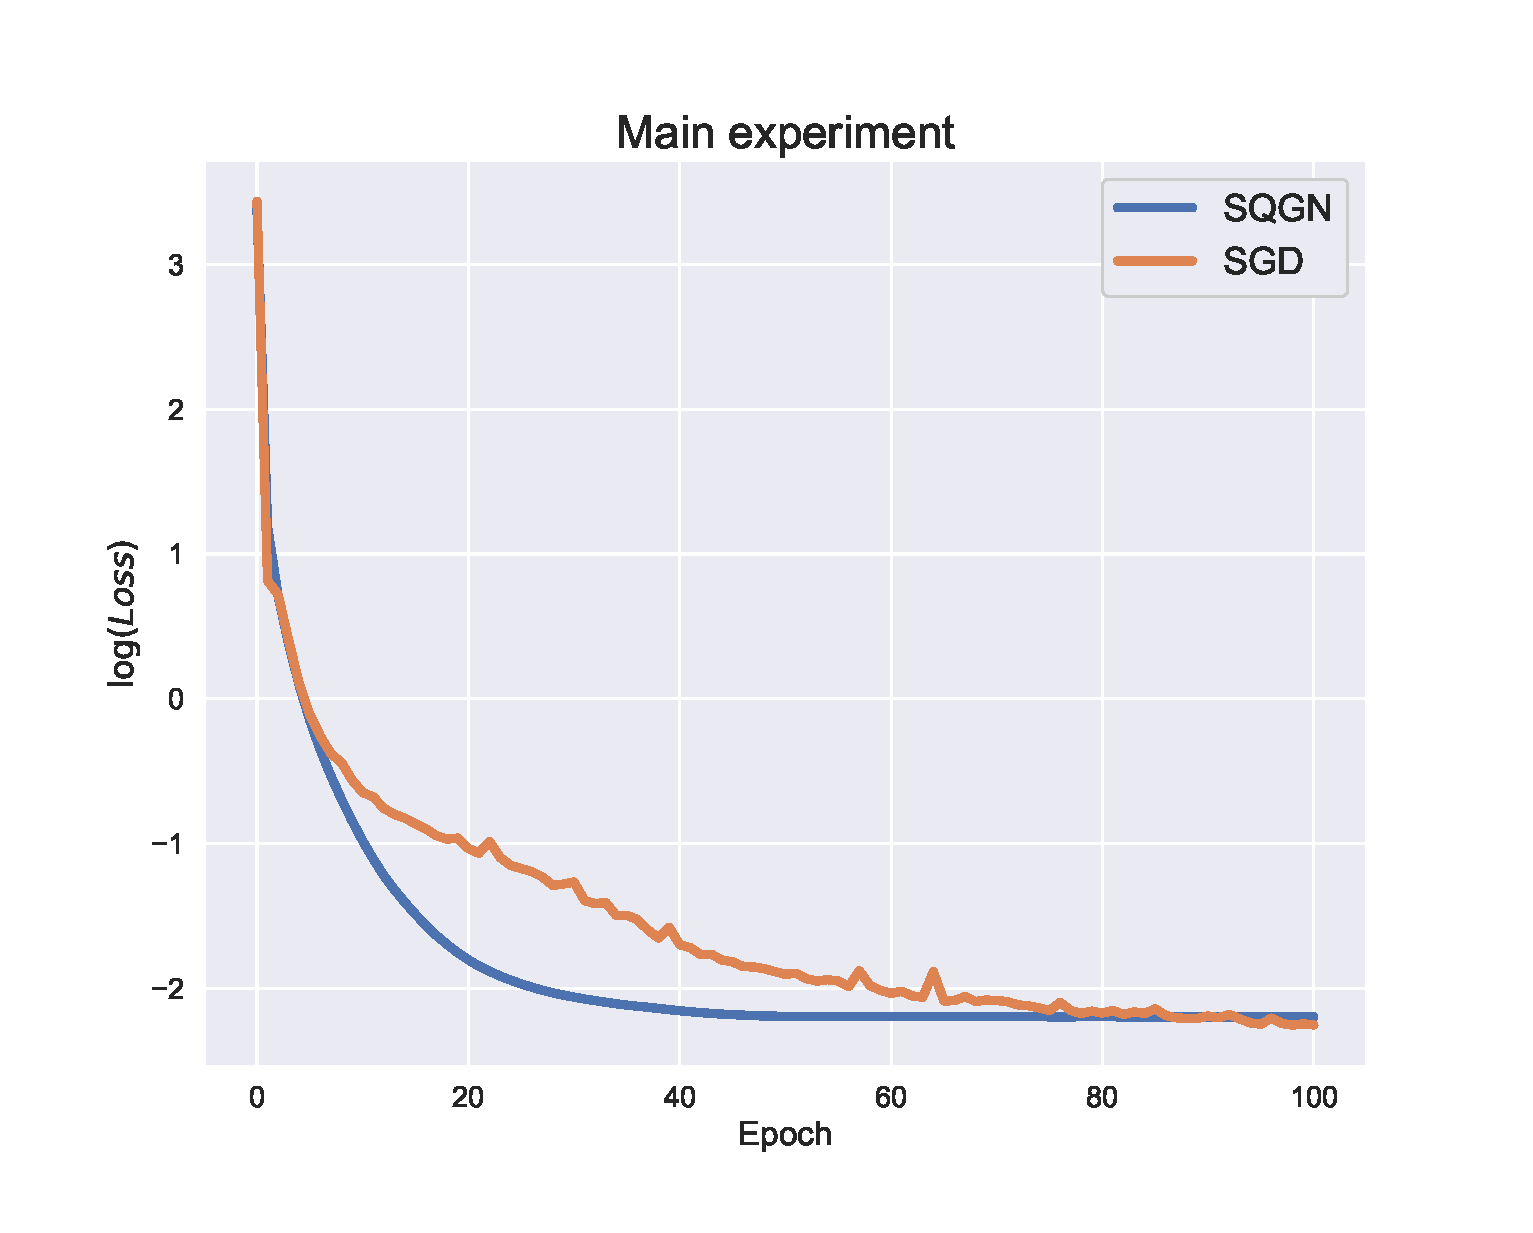
\includegraphics[width=0.9\textwidth]{main_exp.eps}
\end{center}
%Lorem ipsum dolor sit amet, consectetur adipisicing elit, sed do eiusmod tempor incididunt ut labore et dolore magna aliqua. Ut enim ad minim veniam, quis nostrud exercitation ullamco laboris nisi ut aliquip ex ea commodo consequat. Duis aute irure dolor in reprehenderit in voluptate velit esse cillum dolore eu fugiat nulla pariatur. Excepteur sint occaecat cupidatat non proident, sunt in culpa qui officia deserunt mollit anim id est laborum.


%\hrule\medskip
%\Head{Numerical example}\\
%Consider a numerical example with $f(x) = \|Ax - b\|_2^2$
%with $A \in \reals^{10 \times 100}$ and $b \in \reals^{10}$.
%Entries of $A$ and $b$ are generated as independent samples from
%a standard normal distribution.
%Here, we have chosen $\lambda$ using cross validation.
%On this numerical example, the ADMM method converges quickly.
%We give two realizations corresponding to different parameters $A$ and $b$.

\medskip
\hrule\medskip
\Head{Results}\\
\begin{table}[H]
\caption{Result of the main experiment.}
\centering
	\begin{tabular}{ |c|c|c|c|c|c| }
	\hline
	 \multirow{2}{*}{Model} & \multicolumn{4}{c|}{Accuracy, \%} & \multirow{2}{*}{Avg. time/epoch., sec}  \\ \cline{2-5}
	 		& epoch 30 & epoch 50 & ep 70 & ep 100& \\
	 \hline
 	SQN &95.8 & 96.2 & 96.2& 96.2 & 20.3  \\ 
 	SGD &91.5 & 95.1 & 96.0 & 96.6& 9.4 \\ 
 	\hline
\end{tabular}
\end{table}

\medskip
\hrule\medskip
\Head{Conclusion}\\
Our numerical results suggest that SQN converges faster than oLBFGS and SGD. By experimenting with neural networks, we demonstrated that SQN applicable for large-scale optimization problems.

%\medskip
%\hrule\medskip
%\Head{Acknowledgements}\\
%This material is based upon work supported by the
%X Fellowship and my mom.

\bibliographystyle{unsrt}
\bibliography{poster_biblio}
\nocite{*}

\end{textblock}

\end{document}
